\documentclass[11pt, twoside]{book}
\usepackage[full]{leadsheets}
\usepackage[a4paper,  hmargin=1.5cm, vmargin=3cm, head=14pt, foot=50pt]{geometry}
\usepackage{multicol}
\usepackage[polish]{babel}
\usepackage{array}
\usepackage{graphicx}
\usepackage{hyperref}
\usepackage{tocloft}
%\usepackage[toc]{multitoc}  % Odkomentować dla dwukolumnowego spisu treści
\usepackage{fancyhdr}
\usepackage{tikzpagenodes}
\usepackage{titlesec}
\usepackage{tabularx}
\usepackage{adjustbox}
\usepackage{tipa}
\usepackage{ifxetex}
\usepackage[%
    left = \glqq,%
    right = \grqq,%
    leftsub = «,%
    rightsub = »%
]{dirtytalk}

\thispagestyle{empty}

\ifxetex%
    \usepackage{substitutefont}
    \substitutefont{T3}{\rmdefault}{cmr}
\fi

%\usepackage[default]{lato}
%\usepackage[T1]{fontenc}

\selectlanguage{polish}
\DeclareTranslation{Polish}{leadsheets/chorus}{Ref.}
\DeclareTranslation{Polish}{leadsheets/interlude}{Przej.}
\DeclareTranslation{Polish}{leadsheets/lyrics}{tekst}
\DeclareTranslation{Polish}{leadsheets/verse}{Zwr.}
%\DeclareTranslation{Polish}{leadsheets/capo}{Kapo}
\DeclareTranslation{Polish}{leadsheets/fret}{próg}

% Tytuł spisu treści
\addto\captionspolish{\renewcommand*\contentsname{Jakieś piosenki}}

\definesongtitletemplate{custom}{%
    \let\clearpage\relax
    \ifsongmeasuring%
        {\section*}
        {\section}%
        {\songproperty{title}}%
    \begingroup\footnotesize
        \begin{tabular}{%
                @{}
                >{\raggedright\arraybackslash}p{.5\linewidth}
                @{}
                >{\raggedleft\arraybackslash}p{.5\linewidth}
                @{}
            }
            \ifsongproperty{music}{%
                Muzyka: \songproperty{music} \\%
                }{}%
            \ifsongproperty{lyrics}{%
                Tekst: \songproperty{lyrics} \\%
                }{}%
            \ifsongproperty{interpret}{%
                Interpretacja: \songproperty{interpret} \\%
                }{}%
            \ifsongproperty{capo}{%
                & \capo{} \\%
                }{}%
        \end{tabular}%
        \par
    \endgroup
}

\setleadsheets{%
    title-template = custom,
    verse/numbered,
    remember-chords=false,
    align-chords={l},
    capo-nr-format=arabic,
    bar-shortcuts
}
\setchords{%
    minor={lowercase},
    input-notation=german,
    output-notation=german
}

\renewcommand{\chaptermark}[1]{\markboth{#1}{}}

\fancypagestyle{plain}{%
    \fancyhf{}
    \fancyhead[L]{Jakieś piosenki}
    \fancyfoot[LE,RO]{\Large\thepage}
}
\fancypagestyle{szanty}{%
    \pagestyle{plain}
    %\fancyhf{}
    %\fancyhead[L]{Jakieś piosenki}
    \fancyhead[R]{Szanty}
    %\fancyfoot[LE,RO]{\Large\thepage}
    \fancyfoot[LO]{
\includegraphics[height=45pt]{images/kolo.png}}
    \fancyfoot[RE]{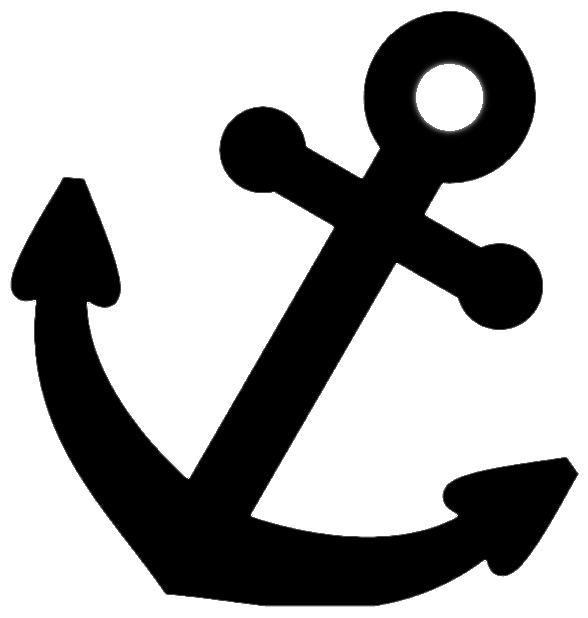
\includegraphics[height=45pt]{images/kotwica.png}}
}
\fancypagestyle{poezja}{%
    \pagestyle{plain}
    \fancyhead[R]{Poezja śpiewana}
    \fancyfoot[LO]{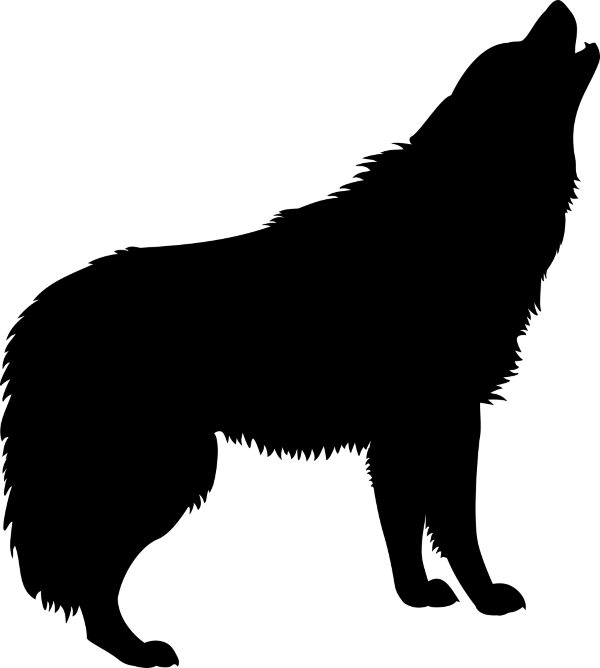
\includegraphics[height=45pt]{images/wilk.png}}
    \fancyfoot[RE]{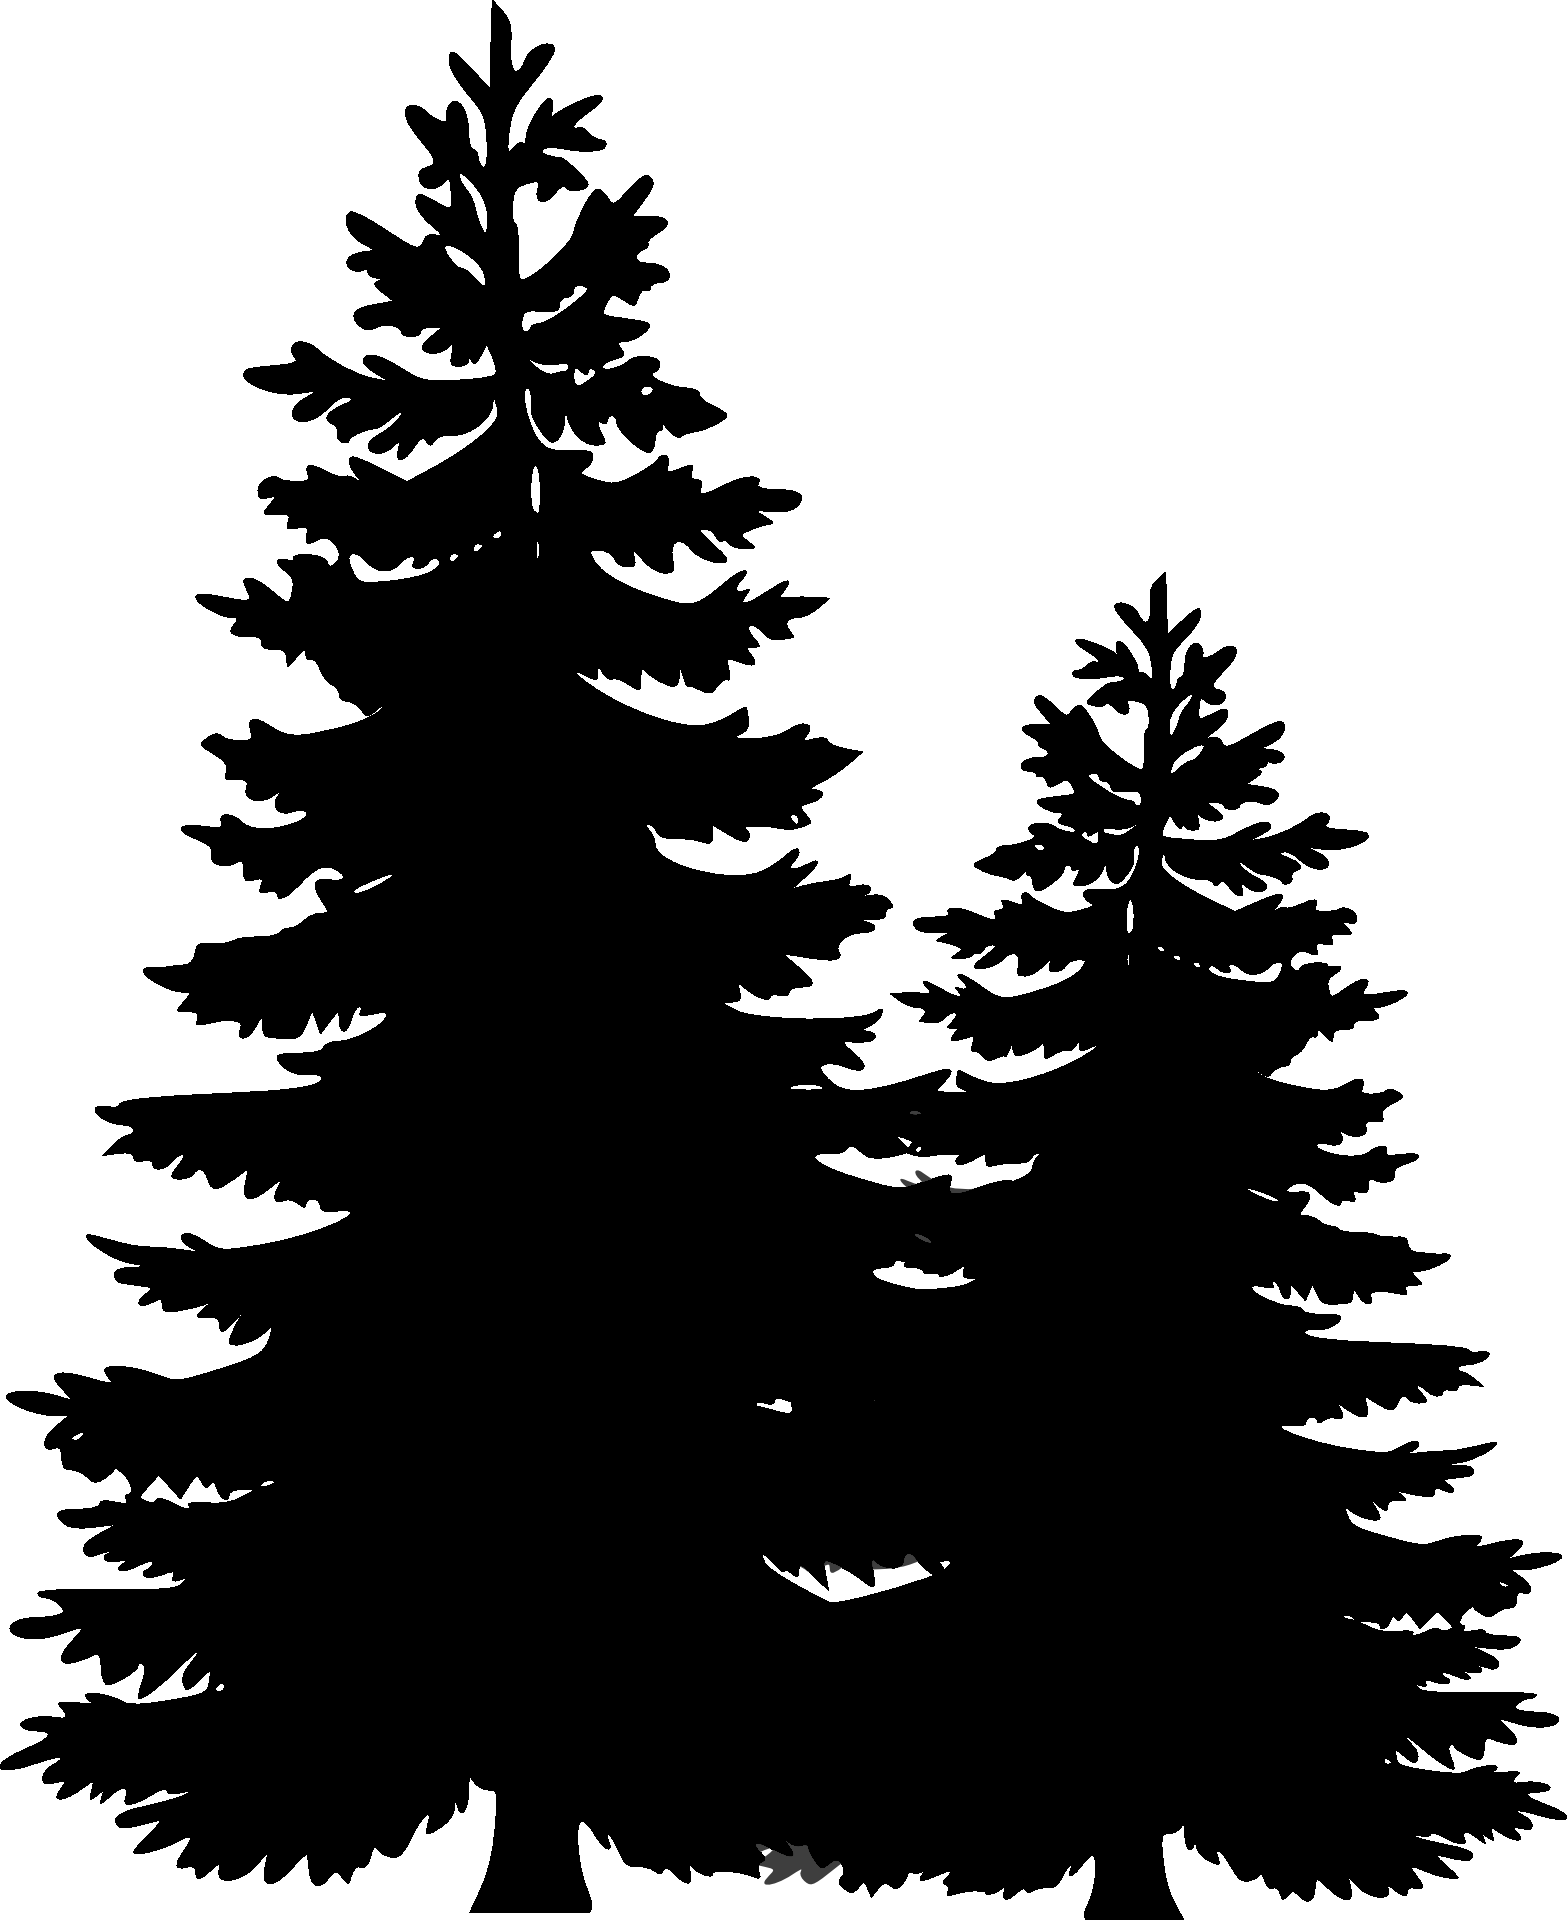
\includegraphics[height=45pt]{images/drzewa.png}}
}
\fancypagestyle{pop}{%
    \pagestyle{plain}
    \fancyhead[R]{Pop}
    \fancyfoot[LO]{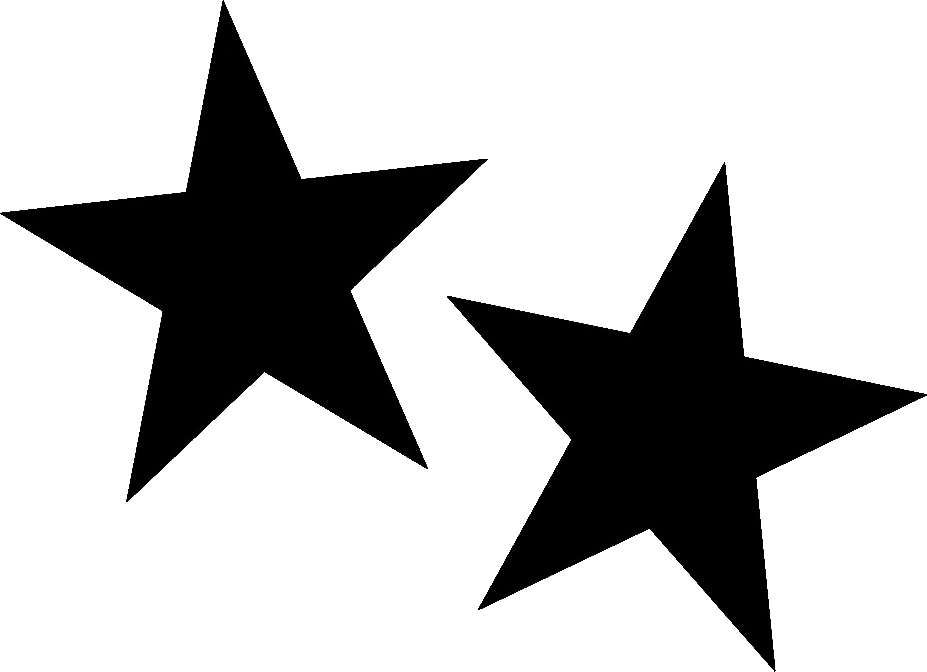
\includegraphics[height=45pt]{images/gwiazdy.png}}
    \fancyfoot[RE]{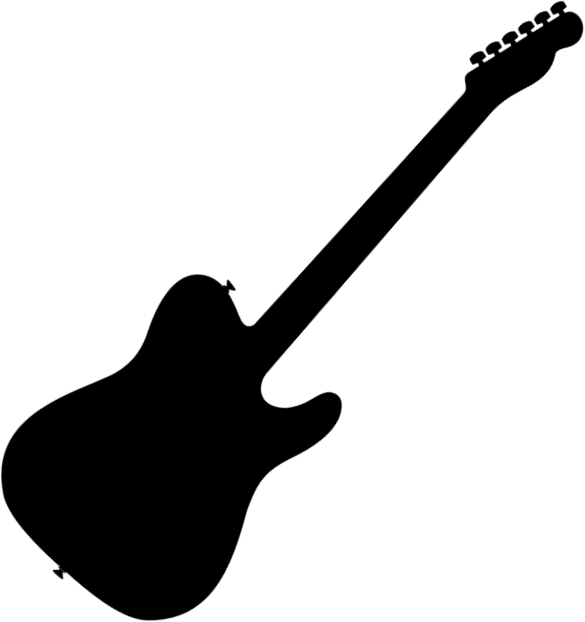
\includegraphics[height=45pt]{images/gitara.png}}
}

\renewcommand{\cftdot}{\ensuremath{\sim}}
\renewcommand{\cftsecleader}{\cftdotfill{\cftdotsep}}

% Usunięcie numeru rozdziału sprzed numeru sekcji
%\renewcommand{\thesection}{\arabic{section}}

\titleformat{\chapter}[block]{\centering\vspace{6cm}}{}{0pt}{\Huge\bfseries}

\newversetype{riff}[name={Riff}, numbered=false, named=true]

\counterwithin*{footnote}{section}
\newcommand{\tqs}{\textquotesingle}

\begin{document}

\begin{titlepage}
    \begin{center}
        \vspace*{5cm}
        
        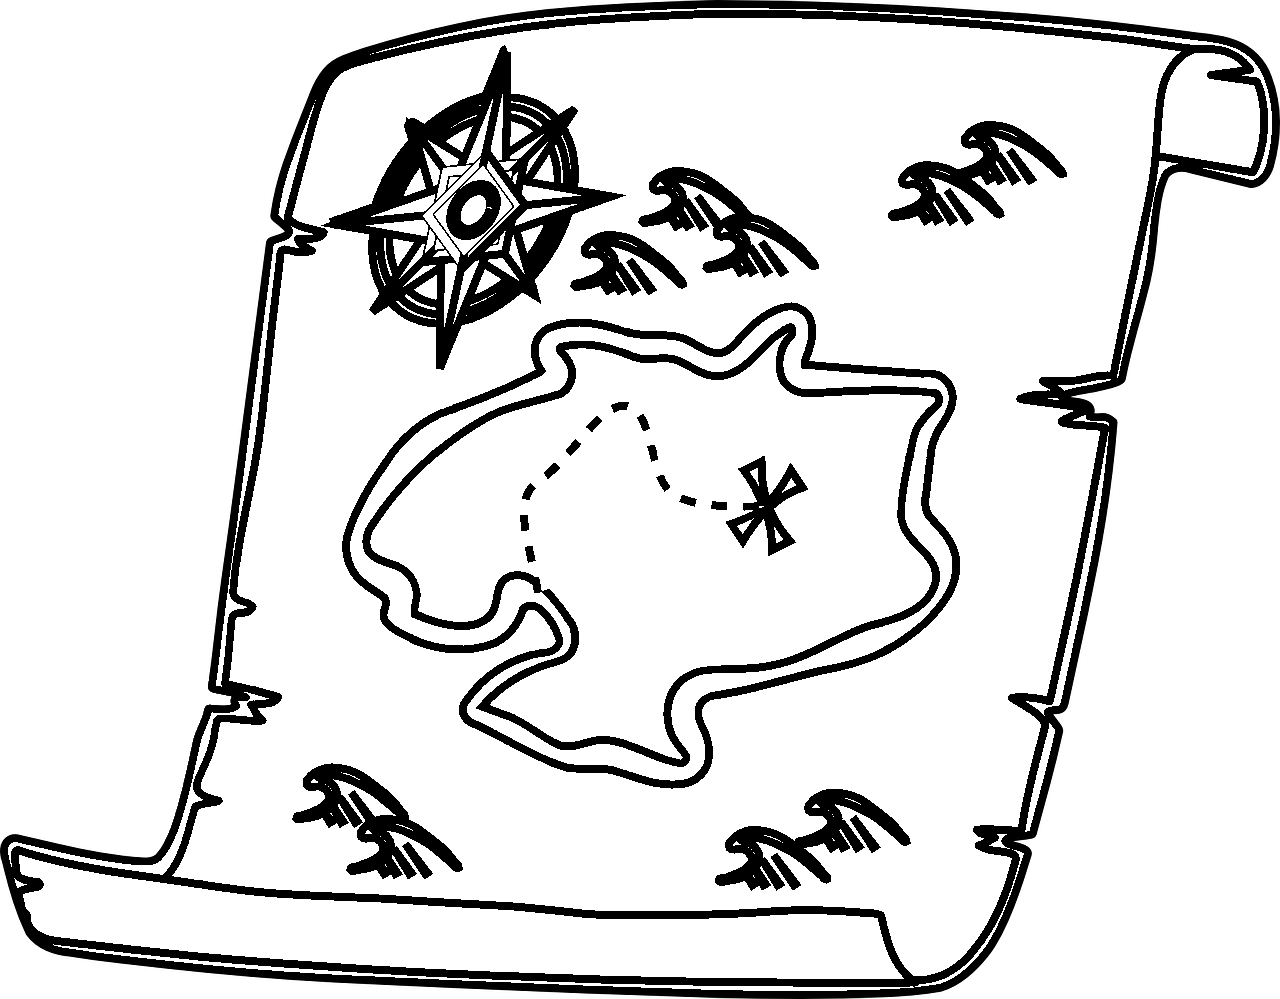
\includegraphics[height=8cm]{images/front-obrazek-aneks.png}

        \vspace{1.5cm}

        \Huge\textbf{Jakieś piosenki}
        
        \vspace{0.3cm}
        \large Aneks dla niegrających na gitarze

        \vspace{0.5cm}
        \large Wydanie pierwsze
        
        \vfill

        \large
        Wydawnictwo Kis Inkris \\
        Warszawa, 2021

        \vspace{0.8cm}

        \footnotesize
        \textit{%
        Gdzie słyszysz śpiew, tam wejdź, tam dobre serce mają \\
        Żli ludzie, wierzaj mi, ci nigdy nie śpiewają} \medskip \\
        Johann Gottfried Seume, \textit{Die Gesänge}
    \end{center}
\end{titlepage}

\tableofcontents
\vfill
\renewcommand{\tabularxcolumn}[1]{>{\small}b{#1}}
\begin{adjustbox}{width={\textwidth}, keepaspectratio}  % Korekta sumarycznej szerokości creditsów i kodu QR
\begin{tabularx}{\textwidth}{%
        @{}
        >{\raggedright\arraybackslash}X
        @{}
        >{\raggedleft\arraybackslash}X
    }
    \footnotesize
    Kamil Dzierżanowski --- opracowanie, skład, korekta

    Paweł Kulig --- opracowanie

    \medskip

    https://github.com/dzierzanowski/spiewnik-szant

    &

    Pobierz śpiewnik online:

    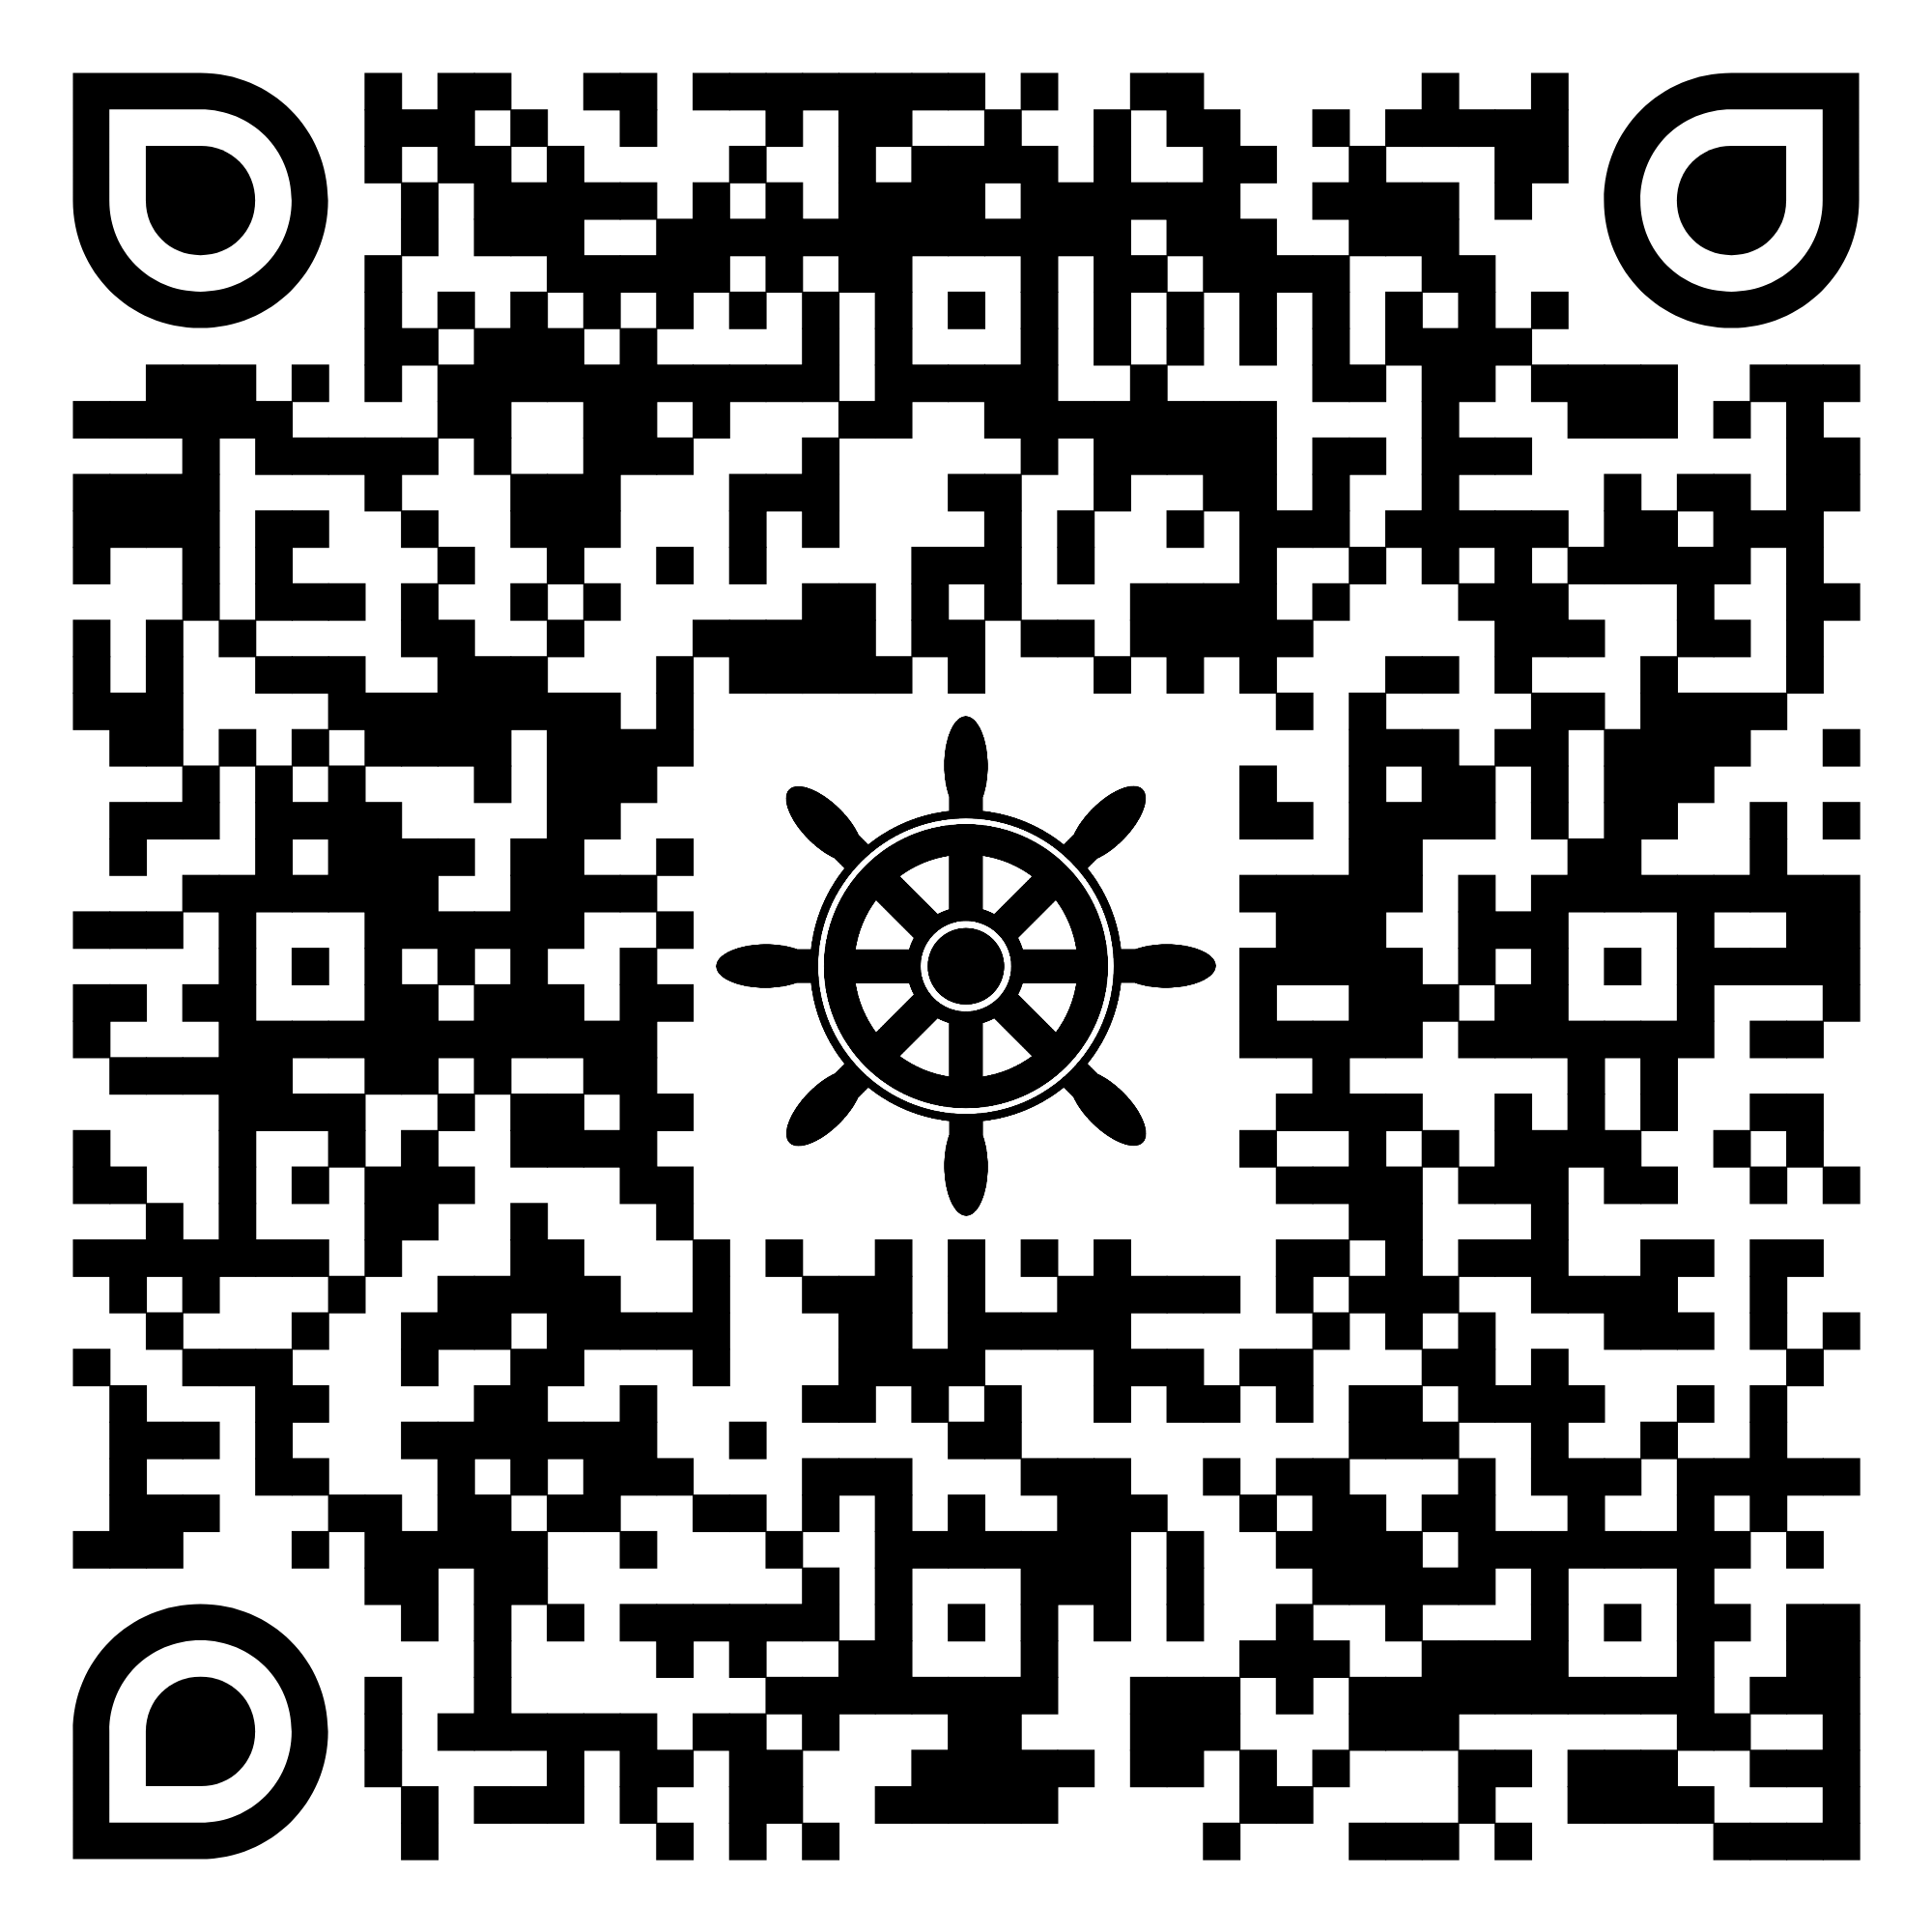
\includegraphics[width=3cm]{images/qr.png}
\end{tabularx}
\end{adjustbox}

\chapter{Szanty}
\begin{center}
    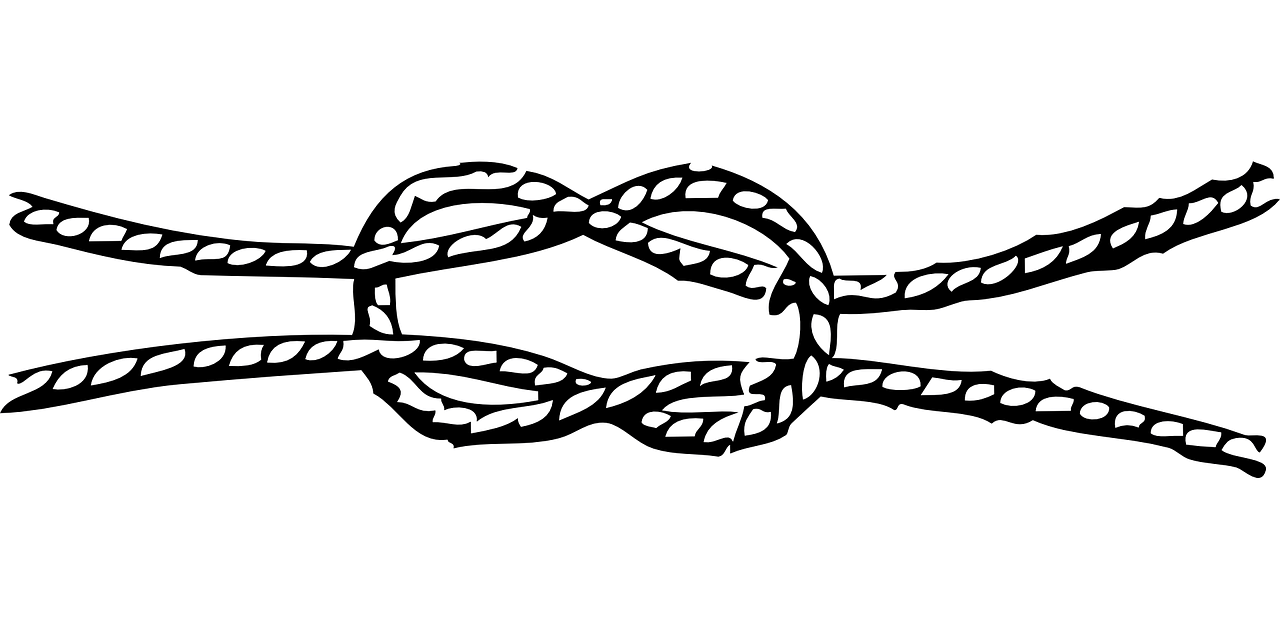
\includegraphics[width=0.5\textwidth]{images/wezel.png}
\end{center}
\pagestyle{szanty}
\setcounter{section}{2}
\newpage
\begin{song}{title={Chłopcy z Botany Bay}, music={Mietek Folk}}
\begin{multicols}{2}
    \begin{verse}
        Już nad ^{c}Hornem ^{B}zapada ^{c}noc \\
        Wiatr na ^{c}żaglach ^{B}położył ^{Eb}się \\
        |: A tam ^{G#}jeszcze ^{B}korsarze na ^*{Eb}Bota ^{B}ny ^{c}Bay | \\
        | Upy^{G#}chają ^{B}zdobycze ^{c}swe :|
    \end{verse}
    \begin{verse}
        Jolly Roger na maszcie już śpi \\
        Jutro przyjdzie z Hiszpanem się bić \\
        A korsarze znużeni na Botany Bay \\
        Za zwycięstwo dziś będa swe pić
    \end{verse}
    \begin{verse}
        Śniady Clark puchar wznosi do ust \\
        \say{Bracia, toast! Niech idzie na dno!} \\
        Tylko Johnny nie pije, bo kilka mil stąd \\
        Otuliło złe morze go
    \end{verse}
    \begin{verse}
        Nie podnosi kielicha do ust \\
        Zawsze on tu najgłośniej się śmiał \\
        Mistrz fechtunku z Florencji ugodził go \\
        Już nie będzie za szoty się brał
    \end{verse}
    \begin{verse}
        W starym porcie zapłacze Margot \\
        Jej kochany nie wróci już \\
        Za dezercję do panny na kei w Brisbane \\
        Oddać musiał swą głowę pod nóż
    \end{verse}
    \begin{verse}
        Tak niewielu zostało dziś ich \\
        Resztę zabrał Neptun pod dach \\
        Choć na ustach wciąż uśmiech, to w sercach lód \\
        W kuflu miesza się rum i strach
    \end{verse}
    \begin{verse}
        To ostatni chyba już rejs \\
        Cios sztyletem lub kula w pierś \\
        Bóg na szkuner w niebiosach zabierze ich \\
        Wszystkich chłopców z Botany Bay
    \end{verse}
    \begin{verse}
        Już nad Hornem zapada noc \\
        Wiatr na żaglach położył się \\
        A tam jeszcze korsarze na Botany Bay \\
        Upychają zdobycze swe
    \end{verse}
\end{multicols}
\begin{center}
    \includegraphics[width=0.7\textwidth]{images/botany\string_bay.png}
\end{center}
\end{song}


\setcounter{section}{4}
\newpage
\begin{song}{title={Dziesięć w skali Beauforta}, music={Krzysztof Klenczon}}
    \begin{multicols}{2}
    \begin{verse}
        Ko^{g}łysał nas zac^{c}hodni wiatr \\
        ^{D7}Brzeg gdzieś za rufą z^{g}ostał \\
        I n^{c}agle ktoś jak p^{g}apier zbladł \\
        ^{A7}Sztorm idzie, panie ^{D}bosman
    \end{verse}
    \begin{chorus}
        A ^*{Eb}bo sm^{B}an tylko ^{Eb}zapiął pł^{B}aszcz \\
        I z^{Eb}aklął: \say{^{D7}Ech, do cz^{g}orta \\
        Nie da^{Eb}ję ła^{F}jbie ż^{B}adnych s^{g}zans} \\
        ^{g}Dziesięć w ^{c}skali ^*{D7}Beau ^{g}forta
    \end{chorus}
    \vfill\null\columnbreak{}
    \begin{verse}
        Z zasłony ołowianych chmur \\
        Ulewa spadła nagle \\
        Rzucało nami w górę, w dół \\
        I fala zmyła żagle
    \end{verse}
    \begin{chorus}
        A bosman tylko zapiął płaszcz\ldots
    \end{chorus}
    \begin{verse}
        Gdzie został ciepły, cichy kąt \\
        I brzegu kształt znajomy \\
        Zasnuły mgły daleki ląd \\
        Dokładnie, z każdej strony
    \end{verse}
    \begin{chorus}
        A bosman tylko zapiął płaszcz\ldots
    \end{chorus}
    \begin{verse}
        O pokład znów uderzył deszcz \\
        I padał już do rana \\
        Piekielnie ciężki to był rejs \\
        Szczególnie dla bosmana
    \end{verse}
    \begin{chorus}
        A bosman tylko zapiął płaszcz \\
        I zaklął: \say{Ech, do czorta \\
        Przedziwne czasem sny się ma} \\
        Dziesięć w skali Beauforta \medskip \\
        Dziesięć w skali Beauforta \\
        Dziesięć w skali Beauforta 
    \end{chorus}
    \end{multicols}
\end{song}


\setcounter{section}{5}  % Jeden mniej niż docelowy
\newpage
\begin{song}{title={Few days}, music={Ryczące Dwudziestki}}
    \medskip
    \begin{adjustbox}{width={\textwidth}, keepaspectratio}
        \includegraphics[width=\textwidth]{songs-alt/ryczace\string_dwudziestki-few\string_days.png}
    \end{adjustbox}
    \begin{info}
        \textit{(beat jak w \say{We Will Rock You})}
    \end{info}
    \begin{multicols}{2}
    \begin{verse}
        O Panie, czemu w ziemi tkwię \\
		Hej raz, hej raz! \\
		I macham szuflą cały dzień? \\
		Hej, na morze czas! 
    \end{verse}
    \begin{chorus}
        Mogę kopać tu dalej \\
		Few days, few days \\
		Mogę kopać przez dni parę \\ 
		Ale wracać chcę  $\times 2$ 
    \end{chorus}
    \begin{verse}
        Tam każdy takie bajdy plótł \\
		Nie raz, nie raz \\
		Przekroczysz Jukon, złota w bród \\
		Hej, na morze czas! 
    \end{verse}
    \begin{chorus}
        Mogę kopać tu dalej\ldots $\times 2$ 
    \end{chorus}
    \begin{verse}
        Wykopię jeszcze parę dziur \\
		Hej raz, hej raz \\
		Wytoczę płonnej skały wór \\
		Hej, na morze czas!
    \end{verse}
    \begin{chorus}
        Mogę kopać tu dalej\ldots $\times 2$ 
    \end{chorus}
    \begin{verse}
        Za żonę tu łopatę mam \\
		Już dość, już dość \\
		A zysk, że jej uzywam sam \\
		Hej, na morze czas!
    \end{verse}
    \begin{chorus}
        Mogę kopać tu dalej\ldots $\times 2$ 
    \end{chorus}
    \begin{verse}
        O Panie nie jest to Twój raj \\
		O nie, o nie \\
		Nadzieję innym głupcom daj \\
		Ja na morze chcę!
    \end{verse}
    \begin{chorus}
        Chociaż już mi wystarczy \\
		Few days, few days \\
		Dam Ci jeszcze jedną szansę \\
		Ale wracać chcę $\times 2$ 
    \end{chorus}
    \end{multicols}
\end{song}


\setcounter{section}{7}
\newpage
\fancyfoot[LO,RE]{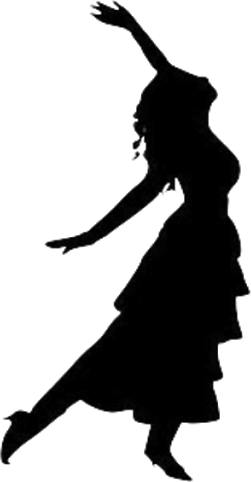
\includegraphics[height=45pt]{images/hiszpanska-dziewczyna.png}}
\begin{song}{title={Hiszpańskie dziewczyny}, music={tradycyjna angielska (Spanish Ladies)}, lyrics={Ryczące Dwudziestki}}
    \begin{intro}
        Żegnajcie nam dziś, hiszpańskie dziewczyny \\
        Żegnajcie nam dziś, marzenia ze snów \\
        Ku brzegom angielskim już rzuszać nam pora \\
        Lecz kiedyś na pewno wró^{G#7}cimy tu z^{c#}nów
    \end{intro}
    \begin{chorus}
        I s^{c#}mak waszych ust, hiszpańskie dziew^{g#}czyny \\
        W noc ^{c#}ciemną i złą nam będzie się ^{H}śnił \\
        Le^{A}niwie pop^{H}łyną znów ^{E}rejsu go^{c#}dziny \\
        Wspom^{A}nienie ust waszych przys^{G#7}porzy nam ^{c#}sił $\times 2$
    \end{chorus}
    \begin{verse}
        Nie^{c#}długo ujrzymy znów w dali Cape ^*{g#}Dead man\footnotemark{} \\
        I Gł^{c#}owę Baranią\footnotemark{} sterczącą wśród wz^{H}górz \\
        I s^{A}tatki sto^{H}jące na ^{E}redzie przed ^{c#}Plymouth \\
        Kla^{A}rować kotwicę naj^{G#7}wyższy czas ^{c#}już
    \end{verse}
    \begin{chorus}
        I smak waszych ust, hiszpańskie dziewczyny\ldots $\times 2$
    \end{chorus}
    \begin{verse}
        I znów białe żagle na masztach rozkwitną \\
        Kurs szyper wyznaczy do Portland i Wight\footnotemark{} \\
        I znów stara łajba potoczy się ciężko \\
        Przez fale, w kierunku na Beachy, Fairlight\footnotemark{}
    \end{verse}
    \begin{chorus}
        I smak waszych ust, hiszpańskie dziewczyny\ldots $\times 2$
    \end{chorus}
    \begin{verse}
        Zabłysną nam bielą skał zęby pod Dover \\
        I znów noc w kubryku wśród legend i bajd \\
        Powoli i znojnie tak płynie nam życie \\
        Na wodach i w portach South Foreland Light\footnotemark{}
    \end{verse}
    \begin{chorus}
        I smak waszych ust, hiszpańskie dziewczyny\ldots $\times 2$
    \end{chorus}
    \footnotetext{Dodman Point, Kornwalia; nie mylić z Cape Diamond, Quebec City --- to po innej stronie oceanu}
    \footnotetext{Ram Head, Kornwalia}
    \footnotetext{Isle of Wight (\textipa{/waIt/})}
    \footnotetext{Beachy Head i Fairlight, East Sussex}
    \footnotetext{wiktoriańska latarnia morska w South Foreland, Kent; nie ustalono, co autor miał na myśli}
\end{song}

\newpage\pagestyle{szanty}
\setcounter{section}{11}
\newpage
\begin{song}{title={La Valette}, interpret={Perły i Łotry}, music={tradycyjna (Le Loup, le Renard et la Belette)}}
    \begin{intro}
        Hej, ho! brakuje oregano! \smallskip \\
        \writechord{B} \writechord{C}
    \end{intro}
    \begin{multicols}{2}
    \begin{chorus}
        ^{g}Pierwszy raz, kiedym stanął w La Valette \\
        ^{B}Bitwy smak poczuły ^{C}usta me \smallskip \\
        Pierwszy raz, kiedym stanął w La Valette \\
        Bitwy smak poczuły usta me \smallskip \\
        Na ^{g}prawo bić, na lewo lać \\
        ^{B}Na kolana Anglio, ^{C}dzisiaj Francji czas \smallskip \\
        Na prawo bić, na lewo lać \\
        Na kolana Anglio, dzisiaj Francji czas $\times 2$
    \end{chorus}
    \smallskip
    \begin{verse}
        Z ^{g}morza widzę Malty brzeg \\
        ^{C}Zbliża się wyzwanie \\
        W ^{g}gardłach armat lont już wrze \\
        ^{C}Kończyć ładowanie! \smallskip \\
        ^{g}Niespokojna żagli biel \\
        ^{C}Trzy kolowy flagi \\
        ^{g}Dalej bracia, równać cel \\
        ^{C}Król zostanie nagi!
    \end{verse}
    \smallskip
    \begin{chorus}
        Pierwszy raz, kiedym stanął w La Valette\ldots $\times 2$
    \end{chorus}
    \vfill\null\columnbreak{}
    \begin{verse}
        Zaraz padnie pierwszy strzał \\
        Już się wiara zbroi \\
        Każdy z nas tej bitwy chciał \\
        Dalej, bić Angoli! \smallskip \\
        Kapitana groźny wzrok \\
        Gromki krzyk załogi \\
        Zaraz zrobi pierwszy krok \\
        \textit{« Vive la France ! »} przeraża wrogów
    \end{verse}
    \begin{interlude}
        \textit{(akordy jak w refrenie)} \\
        \textit{(solo na banjo, jeżeli ktoś ma banjo)}
    \end{interlude}
    \begin{chorus}
        Pierwszy raz, kiedym stanął w La Valette\ldots
    \end{chorus}
    \begin{verse}
        Zapach prochu, błyski szpad \\
        W słońcu lśni fregata \\
        Pierwszy pocisk obok spadł \\
        Dalej, bić psubrata! \smallskip \\
        Dla Francuzów idziem w bój \\
        Za wolności śladem \\
        Trzy kolory to nasz strój \\
        Trzęsie Angol zadem
    \end{verse}
    \begin{chorus}
        Pierwszy raz, kiedym stanął w La Valette\ldots $\times 4$
    \end{chorus}
    \begin{outro}
        Hej, ho! brakuje oregano! \\
        \writechord{B} \writechord{C} \writechord{g}
    \end{outro}
    \vfill\null
    \end{multicols}
\end{song}


\setcounter{section}{17}
\newpage
\fancyfoot[LO,RE]{
\includegraphics[height=45pt]{images/docker.png}}
\begin{song}{title={Pieśń wielorybników}, interpret={EKT Gdynia}, music={tradycyjna (Bonnie Ship the Diamond)}}
    \medskip
    \begin{adjustbox}{width={\textwidth}, keepaspectratio}
        \includegraphics[width=\textwidth]{songs-alt/ekt\string_gdynia-piesn\string_wielorybnikow.png}
    \end{adjustbox}
    \begin{intro}
        a a a d \\
        a e a a $\times 2$
    \end{intro}
    \begin{multicols}{2}
    \begin{verse}
        Nasz D^{a}iament\footnotemark{} prawie g^{e}otów już \\
        W cieśn^{a}inach nie ma kr^{e}y \\
        Na k^{a}ei piękne pa^{e}nny stoją \\
        W o^{d}czach bły^{e}szczą ł^{a}zy \smallskip \\
        Kapitan w niebo wlepia wzrok \\
        Ruszamy lada dzień \\
        Płyniemy tam, gdzie słońca blask \\
        Nie mąci nocy cień
    \end{verse}
    \begin{chorus}
        A więc krz^{a}ycz: \say{^*{e}O-- ^{a}ho!} \\
        Od^{a}wagę w ^{e}sercu mi^{a}ej \\
        Wielo^{a}rybów ^{e}cielska ^{C}groźne ^{G}są \\
        Lecz ^*{F}dosta ^{e}niemy ^{a}je $\times 2$
    \end{chorus}
    \begin{chorus*}
        a a a d \\
        a e a a $\times 2$
    \end{chorus*}
    \vfill\null\columnbreak{}
    \begin{verse}
        Hej panno, po co łzy \\
        Nic nie zatrzyma mnie \\
        Bo prędzej w lodach kwiat zakwitnie \\
        Niż wycofam się \smallskip \\
        No nie płacz mała, wrócę tu \\
        Nasz los nie taki zły \\
        Bo da dukatów wór za tran \\
        I wielorybie kły
    \end{verse}
    \begin{chorus}
        A więc krzycz: \say{O--ho!}\ldots $\times 2$
    \end{chorus}
    \begin{verse}
        Na deku stary wąchał wiatr \\
        Lunetę w ręku miał \\
        Na łodziach co zwisały już \\
        Z harpunem każdy stał \smallskip \\
        I dmucha tu, i dmucha tam  \\
        Ogromne stado w krąg \\
        Harpuny, wiosła, liny brać \\
        I ciągaj brachu ciąg
    \end{verse}
    \begin{chorus}
        A więc krzycz: \say{O--ho!}\ldots $\times 2$
    \end{chorus}
    \begin{interlude}
        \textit{(wolniej)} \\
        I dla ^*{a}wielo ry^{G}ba j^{a}uż \\
        Os^*{e}ta tn^{G}i to dzi^{a}eń \\
        Bo śmi^{a}ały harp^*{C}un n^{G}ik \\
        ^*{F}U de^{G}rza w^{a}eń
    \end{interlude}
    \begin{outro}
        a a a d \\
        a e a a
    \end{outro}
    \end{multicols}
\footnotetext{statek wielorybniczy \say{Diamond}, zmiażdżony przez kry lodowe w Cieśninie Davisa w 1830 r.}
\end{song}

\newpage\pagestyle{szanty}
\setcounter{section}{20}
\newpage
\begin{song}{title={Press gang (Branka)}, music={Cztery Refy}}
    \begin{center}
        \includegraphics[width=\textwidth]{songs-alt/cztery\string_refy-press\string_gang.png}
    \end{center}
\begin{multicols}{2}
    \begin{verse}
        W dół od rzeki, poprzez London Street \\
        Psów królewskich oddział zwarty szedł \\
        Ojczyźnie trzeba dziś świeżej krwi \\
        Marynarzy floty wojennej
    \end{verse}
    \begin{verse}
        A że byłem wtedy silny chłop\\
        W tłumie złowił mnie sierżanta wzrok \\
        W kajdanach z bramy wywlekli mnie \\
        Marynarza floty wojennej
    \end{verse}
    \begin{verse}
        Jak o prawa upominać się \\
        Na gretingu nauczyli mnie \\
        Niejeden krwią wtedy spłynął grzbiet \\
        Marynarza floty wojennej
    \end{verse}
    \begin{verse}
        Nikt nie zliczy ile krwi i łez \\
        Wsiąkło w pokład, gdy się zaczął rejs \\
        Dla chwały twej, słodki kraju mój \\
        Marynarzy floty wojennej
    \end{verse}
    \begin{verse}
        Hen, za rufą miły został dom \\
        Jesteś tylko parą silnych rąk \\
        Dowódca tu twoim bogiem jest \\
        Marynarzu floty wojennej
    \end{verse}
    \begin{verse}
        Gdy łapaczy szyk formuje się \\
        W pierwszym rzędzie możesz ujrzeć mnie \\
        Kto stanie na mojej drodze dziś \\
        \textbf{Łup} stanowi floty wojennej
    \end{verse}
\end{multicols}
\end{song}

\setcounter{section}{23}
\newpage
\begin{song}{title={Santiano}, interpret={Hugues Aufray}, music={tradycyjna}}
    \begin{verse}
        C\tqs est ^{f#}un fameux trois-mâts, fin comme un oise^{E}au \\
        Hissez ^{f#}haut ! « Santi^{E}ano » ! \\
        ^{h}Dix-huit nœuds, quatre ^{E}cents tonne^{h}aux \\
        Je suis ^{f#}fier d\tqs y ^{h}être ^{f#}matelot
    \end{verse}
    \begin{chorus}
        Tiens ^{f#}bon la vague et tiens bon le ^{E}vent \\
        Hissez ^{f#}haut ! « Santi^{E}ano » ! \\
        ^{h}Si Dieu veut, toujours ^{E}droit de^{h}vant \\
        Nous i^{f#}rons jus^{h}qu\tqs à San ^{f#}Francisco
    \end{chorus}
    \begin{verse}
        Je pars pour de longs mois en laissant Margot \\
        Hissez haut ! « Santiano » ! \\
        D\tqs y penser, j\tqs avais le cœur gros \\
        En doublant les feux de Saint-Malo
    \end{verse}
    \begin{chorus}
        Tiens bon la vague et tiens bon le vent\ldots
    \end{chorus}
    \begin{verse}
        On prétend que là-bas, l\tqs argent coule à flots \\
        Hissez haut ! « Santiano » ! \\
        On trouve l\tqs or au fond des ruisseaux \\
        J'en ramènerai plusieurs lingots
    \end{verse}
    \begin{chorus}
        Tiens bon la vague et tiens bon le vent\ldots
    \end{chorus}
    \begin{verse}
        Un jour je reviendrai, chargé de cadeaux \\
        Hissez haut ! « Santiano » ! \\
        Au pays, j\tqs irai voir Margot \\
        À son doigt, je passerai l\tqs anneau
    \end{verse}
    \begin{chorus}
        Tiens bon le cap et tiens bon le flot \\
        Hissez haut ! « Santiano » ! \\
        Sur la mer qui fait le gros dos \\
        Nous irons jusqu\tqs à San Francisco $\times 2$
    \end{chorus}
\end{song}

\setcounter{section}{29}
\newpage
\fancyfoot[LO,RE]{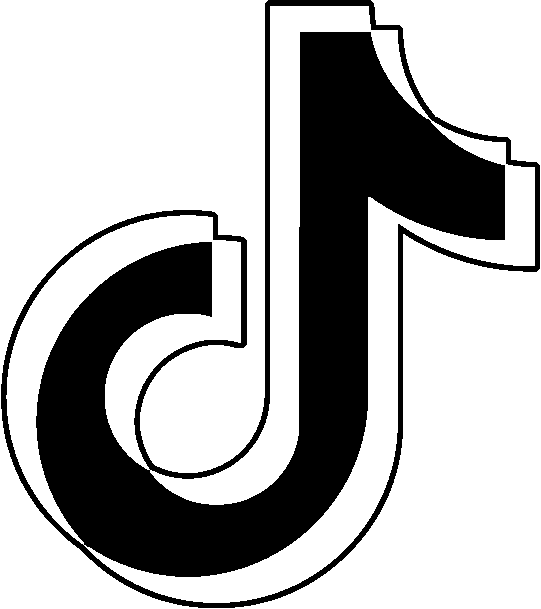
\includegraphics[height=45pt]{images/tiktok.png}}
\begin{song}{title={Wellerman}, music={tradycyjna}}
\begin{multicols}{2}
    \begin{verse}
        There ^{c}once was a ship that put to sea \\
        And the ^{f}name of that ship was the ^{c}Billy o' Tea \\
        The ^{c}winds blew hard, her bow dipped down \\
        ^{B}Blow, me bully boys, ^{c}blow (hoo-ah!)
    \end{verse}
    \begin{chorus}
        ^{G#}Soon may the ^{Eb}Wellerman come \\
        To ^{f}bring us sugar and ^{c}tea and rum \\
        ^{G#}One day, when the ^{Eb}tonguing is done \\
        We'll ^{B}take our ^{G}leave and ^{c}go
    \end{chorus}
    \begin{verse}
        She had not been two weeks from shore \\
        When down on her a right whale bore \\
        The captain called all hands and swore \\
        He'd take that whale in tow (hoo-ah!)
    \end{verse}
    \begin{chorus}
        Soon may the Wellerman come\ldots
    \end{chorus}
    \vfill\null\columnbreak{}
    \begin{verse}
        Before the boat had hit the water \\
        The whale's tail came up and caught her \\
        All hands to the side, harpooned and fought her \\
        When she dived down below (hoo-ah!)
    \end{verse}
    \begin{chorus}
        Soon may the Wellerman come\ldots
    \end{chorus}
    \begin{verse}
        No line was cut, no whale was freed \\
        An' the captain's mind was not on greed \\
        But he belonged to the Whaleman's creed \\
        She took that ship in tow (hoo-ah!)
    \end{verse}
    \begin{chorus}
        Soon may the Wellerman come\ldots
    \end{chorus}
    \begin{verse}
        For forty days or even more \\
        The line went slack then tight once more \\
        All boats were lost, there were only four \\
        And still that whale did go
    \end{verse}
    \begin{chorus}
        Soon may the Wellerman come\ldots
    \end{chorus}
    \begin{verse}
        As far as I've heard, the fight's still on \\
        The line's not cut, and the whale's not gone \\
        The Wellerman makes his regular call \\
        To encourage the captain, crew and all
    \end{verse}
    \begin{chorus}
        Soon may the Wellerman come\ldots $\times 2$
    \end{chorus}
\end{multicols}
\end{song}

\newpage\pagestyle{szanty}

\chapter{Poezja śpiewana}
\begin{center}
    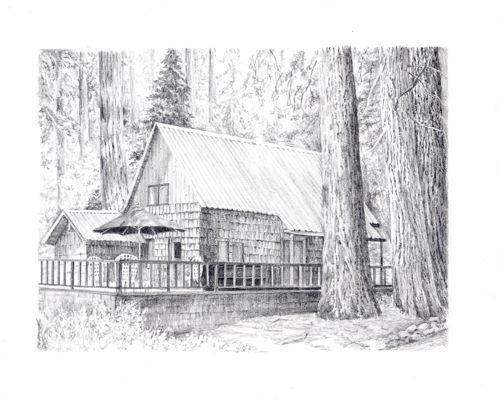
\includegraphics[width=0.5\textwidth]{images/chatka.jpg}
\end{center}
\pagestyle{poezja}
\setcounter{section}{2}
\newpage
\fancyfoot[LO,RE]{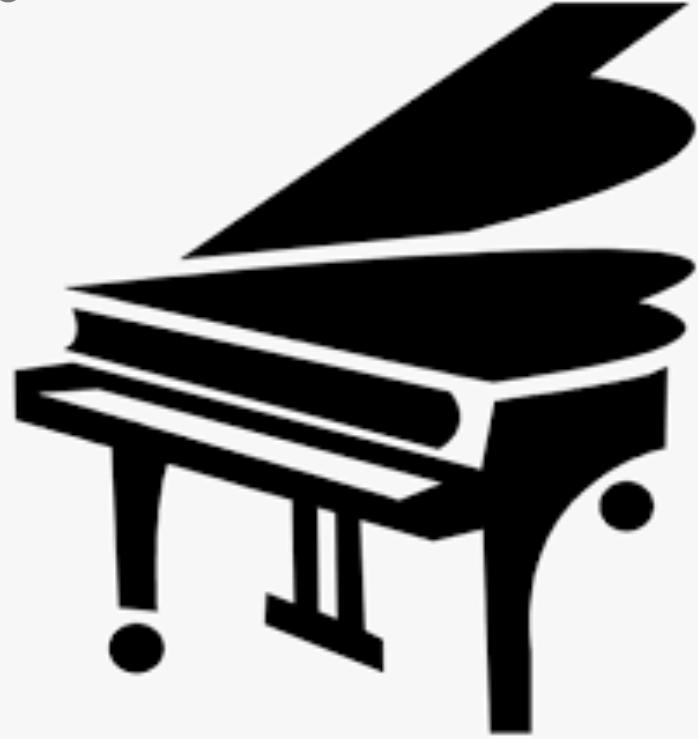
\includegraphics[height=45pt]{images/piano.png}}
\begin{song}{title={Dni, których nie znamy}, music={Jan Kanty Pawluśkiewicz}, lyrics={Marek Grechuta}}
    \begin{intro}
        \textit{(akordy jak w zwrotce)}
    \end{intro}
    \begin{verse}
        ^{c} Tyle było dn^{Eb}i ^{B}do utraty s^{Eb}ił \\
        ^{f}Do utraty t^{C}chu ^{Eb}tyle było chw^{B}il \\
        ^{c}Gdy żałujesz t^{Eb}ych, z kt^{B}órych nie masz n^{Eb}ic \\
        ^{f}Jedno warto zn^{C}ać ^{Eb}jedno tylko wi^{B}edz
    \end{verse}
    \begin{chorus}
        Że ^{G#}ważne są t^{f}ylko te dn^{G7}i, których j^{c}eszcze nie z^*{G#}na ^{B}my ^{Eb} \\
        Ważnych jest kilka tych chwil, tych, na które czekamy \smallskip \\
        Ważne są tylko te dni, których jeszcze nie znamy \\
        Ważnych jest kilka tych chwil, tych, na które czekamy
    \end{chorus}
    \begin{verse}
        Pewien znany ktoś, kto miał dom i sad \\
        Zgubił nagle sens i w złe kręgi wpadł \smallskip \\
        Choć majątek prysł, on nie stoczył się \\
        Wytłumaczyć umiał sobie wtedy właśnie, że\ldots
    \end{verse}
    \begin{chorus}
        Ważne są tylko te dni, których jeszcze nie znamy\ldots
    \end{chorus}
    \begin{interlude}
        ^{c} Jak rozpoznać l^{B}udzi, ^{Eb} których już nie zn^{B}amy \\
        ^{c} Jak pozbierać m^{B}yśli ^{Eb} z tych nieposkład^{B}anych \\
        ^{f} Jak oddzielić n^{C}agle ^{G#} serce od roz^{Eb}umu \\
        ^{c} Jak usłyszeć si^{B}ebie ^{Eb} pośród śpiewu tł^{B}umu \medskip \\
        Jak rozpoznać ludzi, których już nie znamy \\
        Jak pozbierać myśli z tych nieposkładanych \\
        Jak odnaleźć nagle radość i nadzieję \\
        Odpowiedzi szukaj, czasu jest tak wiele
    \end{interlude}
    \begin{chorus}
        Ważne są tylko te dni, których jeszcze nie znamy\ldots
    \end{chorus}
\end{song}

\newpage\pagestyle{poezja}
\setcounter{section}{6}
\newpage
\begin{song}{title={Majster Bieda}, lyrics={Wojciech Bellon}, music={Wolna Grupa Bukowina}}
    \small
    \begin{intro}
        (\writechord{A}) \writechord{D} \writechord{G} \writechord{f#} \writechord{e} $\times 2$ \\
        (\writechord{A}) \writechord{D}
    \end{intro}
    \begin{multicols}{2}
    \begin{verse}
        ^{D} Skąd przychodził, k^{e}to go znał \\
        K^{D}to mu ^{D7}rękę ^{G}podał ki^{A}edy \\
        Nad ^{D}rowem siadał, wyj^{A}mował chleb \\
        ^{e}Serem przekładał i ^{h}dzielił się z psem \\
        ^{A}Tyle wszystkiego, co z ^{G}sobą miał ^{f#}--- ^{e} \\
        ^{A}Majster ^{D}Bieda ^{G} ^{f#} ^{e}
    \end{verse}
    \begin{verse*}
        \writechord{A} \writechord{D}
    \end{verse*}
    \begin{verse}
        Czapkę z głowy ściągał, gdy \\
        Wiatr gałęzie chylił drzewom \\
        Śmiał się do słońca i śpiewał do gwiazd \\
        Drogę bez końca, co przed nim szła \\
        Znał jak pięć palców, jak szeląg zły --- \\
        Majster Bieda
    \end{verse}
    \begin{verse}
        Nikt nie pytał, skąd się wziął \\
        Gdy do ognia się przysiadał \\
        Wtulał się w krąg ciepła jak w kożuch \\
        Zmęczony drogą wędrowiec Boży \\
        Zasypiał długo, gapiąc się w noc --- \\
        Majster Bieda
    \end{verse}
    \vfill\null\columnbreak{}
    \begin{verse}
        Aż nastąpił taki rok \\
        Smutny rok, tak widać trzeba \\
        Nie przyszedł Bieda zieloną wiosną \\
        Miejsce, gdzie siadał, zielskiem zarosło \smallskip \\
        ^{A} I choć niejeden wy^{G}tężał wzrok \\
        Choć ^{A}lato pustym goś^{G}cińcem przeszło \\
        ^{A} Z rudymi liścmi, je^{G}sieni schedą \\
        ^{A}Wiatrem niesiony po^{G}płynął w przeszłość \\
        ^{A}Wiatrem niesiony po^{G}płynął w przeszłość \\
        ^{A}Wiatrem niesiony po^{G}płynął w ^{A}przeszłość --- \\
        ^{A}Majster ^{D}Bieda ^{G} ^{f#} ^{e}
    \end{verse}
    \begin{verse*}
        \writechord{A} \writechord{D} \writechord{G} \writechord{f#} \writechord{e} \\
        \writechord{A} \writechord{D}
    \end{verse*}
    \end{multicols}
\end{song}


\setcounter{section}{11}
\newpage
\begin{song}{title={Świecie nasz}, music={Jan Kanty Pawluśkiewicz}, lyrics={Marek Grechuta}}
\includegraphics[width=\textwidth]{songs-alt/marek\string_grechuta-swiecie\string_nasz.png}
\begin{multicols}{2}
    \begin{intro}
        \writechord{g} \writechord{F} \writechord{Eb} \writechord{d}
    \end{intro}
    \begin{verse}
        ^{g} Pytać zawsze --- ^{F}dokąd, dokąd \\
        ^{Eb} Gdzie jest prawda, ^{d}ziemi sól \\
        ^{g} Pytać zawsze --- ^{F}jak zagubić \\
        ^{Eb} Smutek wszelki, ^{d}płacz i ból
    \end{verse}
    \begin{verse}
        ^{g} Chwytać myśli n^{F}agłe, jasne \\
        ^{B} Szukać tam, gdzie świ^{F/A}atła biel \\
        |: ^{g} W Twoich oczach d^{F}wa ogniki \\
        ^{Eb} Już zwiastują, z^{d}naczą cel :|
    \end{verse}
    \begin{verse*}
        \textit{intro} $\times 2$
    \end{verse*}
    \begin{interlude}
        ^{a} Świecie nasz, ^{g}świecie nasz \\
        Chcę być z Tobą w ^{d}zmowie \\
        ^{F} Z blaskiem Twym, ^{d6}siłą twą \\
        Co mi dasz? Odp^{Esus4}owiedz ^{A}
    \end{interlude}
    \begin{info}
        Świecie nasz --- daj nam \\
        Daj nam wreszcie zgodę \\
        Spokój daj --- zgubę weź \\
        Zabierz ją, odprowadź
    \end{info}
    \begin{info}
        Szukaj dróg gdzie jasny dźwięk \\
        Wśród ogni złych co budzą lęk \\
        Nie prowadź nas, powstrzymaj nas \\
        Powstrzymaj nas w pogoni\ldots
    \end{info}
    \begin{chorus}
        ^{F}Świecie ^{C}nasz \\
        Daj nam wi^{d}ele jasnych dni \\
        ^{a}Świecie n^{F}asz \\
        Daj nam w j^{G}asnym dniu oczekiwanie \medskip \\
        Świecie nasz \\
        Daj ugasić ogień zły \\
        Świecie nasz \\
        Daj nam radość, której tak szukamy \\
        Świecie nasz \\
        Daj nam płomień, stal i dźwięk \\
        Świecie nasz \\
        Daj otworzyć wszystkie ciężkie bramy \\
        Świecie nasz \\
        Daj pokonać każdy lęk \\
        Świecie nasz \\
        Daj nam radość blasku i odmiany! \\
        Świecie nasz \\
        Daj nam cień wysokich traw \\
        Świecie nasz \\
        Daj zagubić się wśród drzew poszumu \\
        Świecie nasz \\
        Daj nam ciszy czarny staw \\
        Świecie nasz \\
        Daj nam siłę krzyku, śpiewu tłumu \\
        Świecie nasz \\
        Daj nam wiele jasnych dni \\
        Świecie nasz \\
        Daj nam w jasnym dniu oczekiwanie \\
        Świecie nasz \\
        Daj ugasić ogień zły \\
        Świecie nasz
    \end{chorus}
    \begin{outro}
        Świecie nasz, świecie nasz \\
        Chcę być z tobą w zmowie \\
        Z blaskiem twym, z siłą twą \\
        Co mi dasz? Odpowiedz
    \end{outro}
\end{multicols}
\end{song}
\fancyfoot[LO,RE]{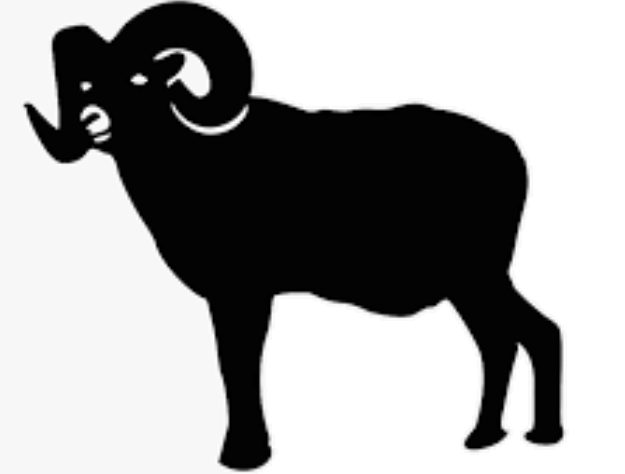
\includegraphics[width=2cm]{images/baran.png}}
\newpage\pagestyle{poezja}

\chapter{Pop}
\begin{center}
    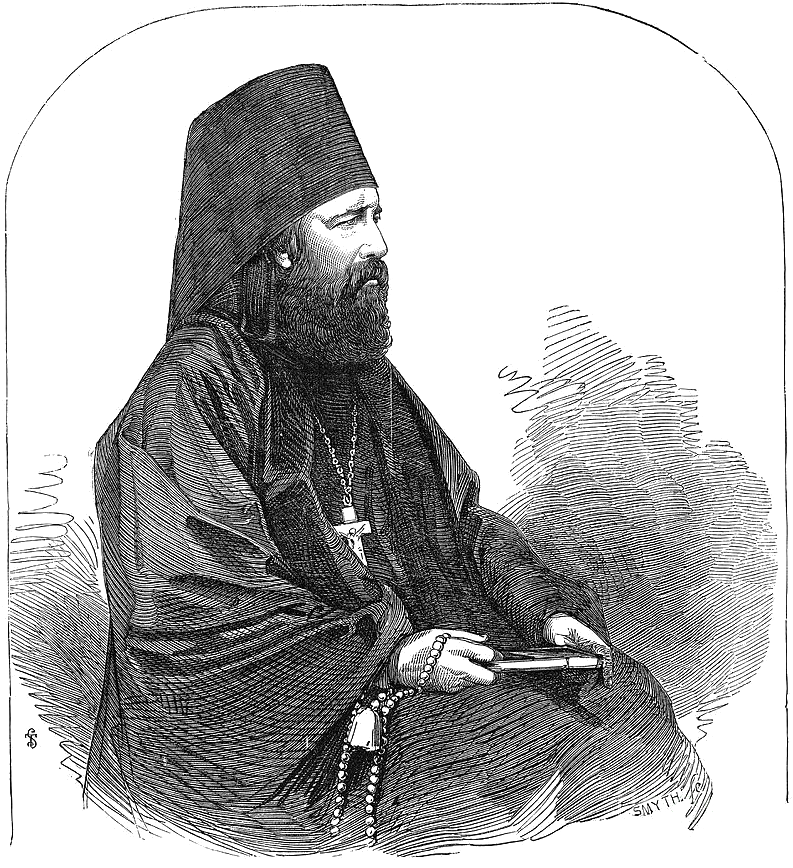
\includegraphics[width=0.4\textwidth]{images/pop.png}
\end{center}
\pagestyle{pop}
\setcounter{section}{0}
\newpage
\begin{song}{title={Byłaś serca biciem}, music={Jerzy Dobrzyński}, interpret={Andrzej Zaucha}}
    \begin{intro}
    \writechord{c} \writechord{B} \writechord{f7} \writechord{f7}
    \end{intro}
    \begin{chorus}
        ^{c}Byłaś serca b^{B}iciem ^{f7} \\
        ^{c}Wiosną, zimą, ż^{B}yciem ^{f7} \\
        ^{c}Marzeń moich e^{B}chem ^{f7} \\
        ^{c}Winem, wiatrem, śmi^{B}echem ^{f7}
    \end{chorus}
    \begin{verse}
        Ostatnio w ^{c}mieście mym tramwaje ^{B}po północy b^{f7}łądzą \\
        Rozkładem n^{c}ocnych tras piekielne ^{B}jakieś moce rz^{f7}ądzą \\
        Nie wiedzieć ^{c}czemu wciąż rozkł^{B}ady jazdy ta^{f7}k zmieniają \\
        Że prawie k^{c}ażdy tramwaj ^{B}pod twym oknem ^{f7}nocą staje
    \end{verse}
      \begin{chorus}
        Byłaś serca biciem\ldots
    \end{chorus}
    \begin{verse}
        Ostatnio słońca mniej, ostatnio noce bardziej ciemne \\
        Już nawet księżyc drań o tobie nie chce gadać ze mną \\
        W kieszeni grosze dwa, w kieszeni na dwa szczęścia grosze \\
        W tym jednak losu żart, że ja obydwa grosze noszę
    \end{verse}
    \begin{chorus}
        Byłaś serca biciem\ldots
    \end{chorus}
    \begin{interlude}
        ^{Ab}Ktoś p^{f7}ytał jak się m^{Eb}asz, j^{c}ak się czujesz \\
        ^{Ab}Ktoś, z k^{f7}im rok w wojnę g^{Eb}rasz wycze^*{g}ku ^{C}je \\
        ^{Ab}Ktoś, k^{f7}to nocami, u^{Eb}licami, t^{c}ramwajami \\
        ^{Ab}Pod twe okno m^{f7}knie, gdzie spo^*{F}ty ^{Gb}ka ^{G}mnie
    \end{interlude}
    \begin{chorus}
        Byłaś serca biciem\ldots
    \end{chorus}
    \begin{interlude}
        Ktoś pytał jak się masz\ldots
    \end{interlude}
\end{song}


\setcounter{section}{2}
\newpage
\begin{song}{title={Hydropiekłowstąpienie}, music={Lao Che}}
\small
\begin{multicols}{2}
    \begin{intro}
        \writechord{f#5} \writechord{a5} \writechord{d5} \writechord{c#5}
    \end{intro}
    \begin{riff}
        \writechord{f#} \writechord{C#7} \writechord{f#} \writechord{C#7} $\times 8$
    \end{riff}
    \begin{verse}
        Słuchaj, Noe, chciałbym na słówko \smallskip \\
        Wiesz, tak między nami, to \\
        Jestem człowiekiem zaniepokojony \\
        By rzec: rozczarowany \smallskip \\
        Bo miałem ambicję stworzyć \\
        Taką rezolutną rasę \smallskip \\
        A wyście to tak po ludzku \\
        Po ludzku, spartolili \smallskip \\
        Jestem piekielnie sfrustrowany
    \end{verse}
    \begin{interlude}
        Płyń, płyń, Noe, płyń i żyj, a utop to, kim byłeś \\
        Płyń, płyń, Noe, płyń i żyj, jak nawet nie śniłeś
    \end{interlude}
    \begin{verse}
        Wiesz sam, jak nie lubię radykałów \smallskip \\
        Ale, na Boga, nie spałem całą noc \\
        I podjąłem decyzję \smallskip \\
        Zsyłam na Ziemię potop \\
        Mój mały Noe \smallskip \\
        Mój ptysiu miętowy, zsyłam potop \\
        Potop!
    \end{verse}
    \begin{riff}
        \writechord{f#} \writechord{C#7/G#} \writechord{A} \writechord{C#7/G#} 
    \end{riff}
    \begin{chorus}
        Utopię waszą utopię \\
        Utopię waszą utopię, ja\ldots \smallskip \\
        Utopię waszą utopie \\
        Utopię w potopie \\
        Zarządzam pełne zanurzenie \smallskip \\
        Utopię waszą utopie \\
        Utopię w potopie \\
        Hydropiekłowstąpienie
    \end{chorus}
    \begin{verse}
        Zatem, utonie wszystko: \smallskip \\
        Drogi i mosty kołowe \\
        Urzędy skarbowe \\
        Gospodarstwa domowe \smallskip \\
        Powiadam: wszystko \\
        Za wyjątkiem ciebie, chłopaku \\
        Wypływasz jutro \\
        Mandżur pakuj!
    \end{verse}
    \begin{chorus}
        Utopię waszą utopię\ldots
    \end{chorus}
    \begin{interlude}
        \writechord{f#5} \writechord{a5} \writechord{d5} \writechord{c#5} $\times 4$ \medskip \\
        Płyń, płyń, Noe, płyń i żyj, a utop to, kim byłeś \\
        Płyń, płyń, Noe, płyń i żyj, jak nawet nie śniłeś
    \end{interlude}
    \begin{verse}
        Wybrałem ciebie, bo\ldots \\
        Tak właściwie, to nie wiem \\
        Dlaczego ciebie wybrałem \smallskip \\
        Chciałem tylko, żebyś był fajny \\
        I żeby ktoś kiedyś mógł powiedzieć: \smallskip \\
        \say{Był Noe \\
        Noe --- gość, co się czasem spinał \smallskip \\
        Ale uwierzył, i gdy szedł po gnoju \\
        Smród już się go nie imał!}
    \end{verse}
    \begin{chorus}
        Płyń, chłopaku, płyń \\
        Płyń, nie odwracaj główki chłopaku, ty płyń \\
        A ja\ldots \smallskip \\
        Utopię waszą utopię \\
        Utopię w potopie \\
        Zarządzam pełne zanurzenie \smallskip \\
        Utopię waszą utopię \\
        Utopię w potopie \\
        Hydropiekłowstąpienie \medskip \\
        \writechord{f#5} \writechord{a5} \writechord{d5} \writechord{c#5} $\times 2$
    \end{chorus}
\end{multicols}
\end{song}


\setcounter{section}{12}
\newpage
\fancyfoot[LO,RE]{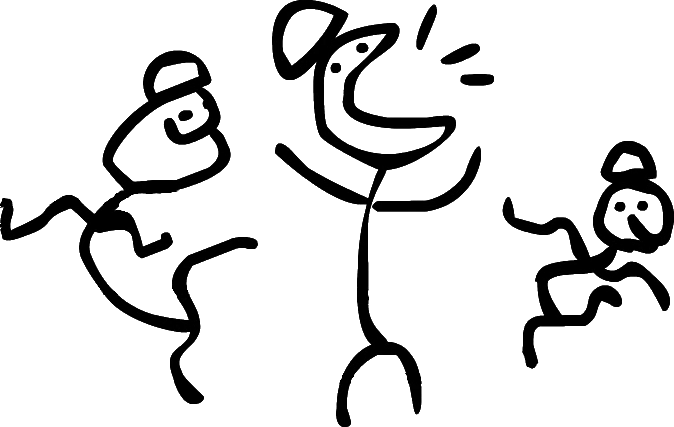
\includegraphics[height=45pt]{images/hutnicy.png}}
\begin{song}{title={Piosenka o hucie}, lyrics={Jakub \say{Dem3000} Dębski}, music={Romek Buga}}
    \begin{intro}
        \say{Czasami w hu^{Ebmaj7}cie spotykamy się wszyscy i pracujemy tam \\
        A ^{f7}czasami nie, czasami śpiewamy piosenki, na przykład moją ulubio-- \\
        Moją ^{B7}ulubioną piosenkę} --- pomyślał sobie, przypomniał sobie swoją ulubioną piosenkę:
    \end{intro}
    \begin{chorus}
        ^{Ebmaj7}Hej! ^*{c7} Otrzymy ^{f7}wanie me^{B7}tali \\
        Z r^{Ebmaj7}ud i z^{c7}łomu ^{f7} ^{B7} \\
        To jest ^{Ebmaj7}to, co ^{c7}lubię naj^{f7}bardziej ^{B7} \\
        To jest ^{Ebmaj7}to, co ^{c7}lubię naj^{f7}bardziej \\
        ^{B7}Wytapiać sz^{Ebmaj7}kło --- i prze^{c7}twarzać produkty sz^{f7}klane ^{B7} \\
        Praca w ^*{Ebmaj7}hu--- ^*{c7}uc ^{f7}ie ^{B7} \\
        Praca w hu^{Ebmaj7}cie
    \end{chorus}
\end{song}

\newpage\pagestyle{pop}
\setcounter{section}{21}
\newpage
\begin{song}{title={Trudno nie wierzyć w nic}, music={Raz Dwa Trzy}}
    \begin{adjustbox}{width={\textwidth}, keepaspectratio}
        \includegraphics[width=\textwidth]{songs-alt/raz\string_dwa\string_trzy-trudno\string_nie\string_wierzyc\string_w\string_nic.png}
    \end{adjustbox}
    \begin{multicols}{2}
     \begin{verse}
        ^{e} ^{G/D}Zapyta Bóg ^{C(5-)} w swym ^{H}niebie \\
        ^{e} Co ^{G/D}dałem Mu, ^{C(5-)} od ^{H}siebie \\
        ^{e} ^{G/D}Wierzyłem i ^{C(5-)} ^{H}kochałem \\
        ^{e} I ^{G/D}byłem tym, ^{C(5-)} kim ^{H}chciał bym ^{C}był \smallskip \\
        I ż^{D}yłem jak, ^{C}chciał bym żył \\
        I ^{D}byłem, kim mi^{H}ałem być
    \end{verse}
    \begin{interlude}
        \textit{(intro)} $\times 1$
    \end{interlude}
    \begin{verse}
        Odpowiem Mu od siebie \\
        Że spłacę dług tym lepiej \\
        Tym bardziej, bo wiedziałem \\
        Co znaczy, że nadziei brakowało mi \medskip \\
        ^{C} I ^{D}kilku chwil, kilku ^{G}dobrych chwil ^{C} \\
        Może powie, ^{a}to niepotr^{H}zebne słowa
    \end{verse}
    \begin{chorus}
        ^{e} ^{G/D} Trudno nie w^{C(5-)}ierzyć w nic ^{H} \\
        Trudno nie wierzyć w nic \\
        Trudno nie wierzyć w nic \\
        Trudno nie wierzyć w nic
    \end{chorus}
    \begin{solo}
        C D $\times 8$
    \end{solo}
    \begin{verse}
        Zapyta Bóg w swym niebie \\
        Jak spłacę dług --- ja nie wiem \\
        Wierzyłem i kochałem \\
        I byłem tym, kim chciał bym był
    \end{verse}
    \begin{chorus}
        Trudno nie wierzyć w nic \\
        Trudno nie wierzyć w nic
    \end{chorus}
    \begin{outro}
        \textit{(intro)} $\times 1$
    \end{outro}
    \end{multicols}
\end{song}


\setcounter{section}{22}
\newpage
\begin{song}{title={Warszawa}, music={T.Love}}
    \normalsize
    \begin{intro}
        \writechord{E} \writechord{A} $\times 2$
    \end{intro}
    \begin{multicols}{2}
    \begin{verse}
        Za ^{H}oknem zimowo zaczyna się dzień \\
        Za^{c#}czynam kolejny dzień ż^{A}ycia \\
        Wyg^{H}lądam przez okno, na oczach mam sen \\
        A ^{c#}Grochów się budzi z prze^{A}picia \medskip

        Wypity alkohol uderza w tętnice \\
        Autobus tapla się w śniegu \\
        Zza szyby oglądam betonu stolicę \\
        Już jestem na drugim jej brzegu
    \end{verse}
    \begin{chorus}
        Gdy ^{E}patrzę w twe ^{H}oczy zmę^{A}czone jak moje \\
        To ^{E}kocham to ^{H}miasto zmę^{A}czone jak ja \\
        Gdzie ^{E}Hitler i Sta^{H}lin zro^{A}bili, co swoje \\
        Gdzie ^{E}wiosna spa^{H}liną odd^{A}ycha
    \end{chorus}
    \begin{interlude}
        \writechord{E} \writechord{A} $\times 2$
    \end{interlude}
    \vfill\null\columnbreak{}
    \begin{verse}
        Krakowskie Przedmieście zalane jest słońcem \\
        Wirujesz jak obłok, wynurzasz się z bramy \\
        A ja jestem głodny, tak bardzo głodny \\
        Kochanie, nakarmisz mnie snami \medskip

        Zielony Żoliborz, pieprzony Żoliborz \\
        Rozkwita na drzewach, na krzewach \\
        Ściekami z rzeki kompletnie pijany \\
        Chcę krzyczeć, chcę ryczeć, chcę śpiewać
    \end{verse}
    \begin{chorus}
        Gdy patrzę w twe oczy zmęczone jak moje\ldots \smallskip

        \writechord{H} \writechord{c#} \smallskip

        Gdy patrzę w twe oczy zmęczone jak moje\ldots
    \end{chorus}
    \begin{interlude}
        \writechord{H} \writechord{H} \writechord{c#} \writechord{A} $\times 4$ \textit{(jak w zwrotce)} \medskip \\
        \writechord{E} \writechord{H} \writechord{E} \\
        (\writechord{H})\writechord{E} \writechord{A} \writechord{H} \\
        \writechord{E} \writechord{H} \writechord{E} \medskip \\
        \writechord{E} \writechord{H} \writechord{E} \\
        (\writechord{H})\writechord{E} \writechord{A} \writechord{H} \\
        \writechord{A}
    \end{interlude}
    \begin{verse}
        Jesienią zawsze zaczyna się szkoła \\
        A w knajpach zaczyna się picie \\
        Jest tłoczno i duszno, olewa nas kelner \\
        I tak skończymy o świcie \medskip

        Jesienią zawsze myślę o latach \\
        Tak starych, jak te kamienice \\
        Jesienią o zmroku przechodzę z tobą \\
        Przez pełne kasztanów ulice
    \end{verse}
    \begin{chorus}
        I patrzę w twe oczy zmęczone jak moje \\
        I kocham to miasto zmęczone jak ja \\
        Gdzie Hitler i Stalin zrobili, co swoje \\
        Gdzie wiosna spaliną oddycha $\times 2$
    \end{chorus}
    \begin{outro}
        \writechord{H} \writechord{E}
    \end{outro}
    \end{multicols}
\end{song}



% Ostatnia strona parzysta pusta, żeby nie było tekstu na odwrocie
\clearpage{\mbox{}\pagestyle{empty}\cleardoublepage}

\end{document}
